\RequirePackage{docswitch}
% \flag is set by the user, through the makefile:
%    make note
%    make apj
% etc.
\setjournal{\flag}

\documentclass[\docopts]{\docclass}

% You could also define the document class directly
%\documentclass[]{emulateapj}

% Custom commands from LSST DESC, see texmf/styles/lsstdesc_macros.sty
\usepackage{lsstdesc_macros}
\usepackage{rotating}
\usepackage{graphicx}
\usepackage{diagbox}
\usepackage{multirow}
\usepackage{adjustbox}
\usepackage{comment}
\usepackage{mathtools}

%\usepackage{pdflscape}
\graphicspath{{./}{./figures/}}
\bibliographystyle{apj}

% Add your own macros here:
\newcommand{\snrb}{\mbox{$SNR^b$}}
\newcommand{\snrbmin}{\mbox{$SNR^b_{min}$}}
\newcommand{\snrg}{\mbox{$SNR^g$}}
\newcommand{\snrr}{\mbox{$SNR^r$}}
\newcommand{\snri}{\mbox{$SNR^i$}}
\newcommand{\snrz}{\mbox{$SNR^z$}}
\newcommand{\snry}{\mbox{$SNR^y$}}
\newcommand{\z}{{$z$}}
\newcommand{\bu}{{$u$}}
\newcommand{\bg}{{$g$}}
\newcommand{\br}{{$r$}}
\newcommand{\bi}{{$i$}}
\newcommand{\bz}{{$z$}}
\newcommand{\by}{{$y$}}
\newcommand{\salt}{SALT2}
\newcommand{\xnorm}{$x_0$}
\newcommand{\strech}{$x_1$}
\newcommand{\snstrech}{\mbox{$x_1$}}
\newcommand{\col}{$c$}
\newcommand{\daymax}{$T_0$}
\newcommand{\sigc}{\mbox{$\sigma_c$}}
\newcommand{\sigmu}{\mbox{$\sigma_\mu$}}
\newcommand{\zlim}{\mbox{$z_{lim}$}}
\newcommand{\zlimfaint}{\mbox{$z_{lim,faint}^{SN}$}}
\newcommand{\cosmos}{{\sc COSMOS}}
\newcommand{\elais}{{\sc ELAIS-S1}}
\newcommand{\xmm}{{\sc XMM-LSS}}
\newcommand{\cdfs}{{\sc CDF-S}}
\newcommand{\adfa}{{\sc ADF-A}}
\newcommand{\adfb}{{\sc ADF-B}}
\newcommand{\adfs}{{\sc EUCLID/Roman}}
\newcommand{\euclid}{{\sc EUCLID}}
\newcommand{\romanspace}{{\sc Roman Space Telescope}}
\newcommand{\wfirst}{{\sc WFIRST}}
\newcommand{\sne}{{SNe Ia}}
\newcommand{\degsq}{{deg$^2$}}
\newcommand{\nsn}{{$N_{SN}^{z\leq z_{lim}}$}}
\newcommand{\nsncomp}{{$N_{SN}^{z\leq z_{complete}}$}}
\newcommand{\sumnsncomp}{{$\sum\limits_{Npixels} N_{SN}^{z\leq z_{complete}}$}}
\newcommand{\zcomp}{\mbox{$z_{complete}$}}
\newcommand{\zcompb}{\mbox{$z_{complete}^{0.95}$}}
\newcommand{\snfaint}{\mbox{$(\snstrech,\sncolor)=(-2.0,0.2)$}}
\newcommand{\snx}{\mbox{$x_0$}}
\newcommand{\sncolor}{\mbox{$c$}}
\newcommand{\redshift}{\mbox{$z$}}
\newcommand{\per}{$\%$}
\newcommand{\seq}{$\sim$}
\newcommand{\nvisits}{$N_{visits}$}
\newcommand{\nvisitsb}{\mbox{$N_{visits}^b$}}
\newcommand{\sumnvisitsb}{\mbox{$\sum\limits_{b}N_{visits}^b$}}
\newcommand{\nvisitsbmin}{\mbox{$N_{visits,min}^b$}}
\newcommand{\nvisitsy}{$N_{visits}^y$}
\newcommand{\nvisitsall}{$N_{visits}^g,N_{visits}^r,N_{visits}^i,N_{visits}^z,N_{visits}^y$}
\newcommand{\ddfscen}[1]{RDD\_#1}
\newcommand{\osfamily}[1]{{\it #1}}
\newcommand{\doffset}{tdo}

% ======================================================================

\begin{document}

\title{LSST Deep Drilling program and Supernovae}

\maketitlepre

\begin{abstract}

  Write abstract here.

\end{abstract}

% Keywords are ignored in the LSST DESC Note style:
\dockeys{}

\maketitlepost

% ----------------------------------------------------------------------
% 

\section{Introduction}
\label{sec:intro}
Type Ia supernovae(\sne) are transient astronomical events resulting from a powerful and luminous explosion of a white dwarf. They are identified by their brightness evolution, with a luminosity peak about 15 days after explosion, and a slow decrease lasting up to few months. \sne~can be used as standard candles to determine cosmological distances. They are included in a Hubble diagram, one is the most statistically efficient approach to constraint the Dark Energy equation of state (\citealt{Betoule_2014,Scolnic_2018}).
\par
The stated ambition of the LSST Supernovae program is to maximize the sample size of well-measured type Ia supernovae while reducing systematic uncertainties on cosmological parameters. Increasing the statistics in the Hubble diagram requires (1) advances in the measurement of the distances (i.e.  a control at the per-mil level of the photometry and survey flux calibration, and a progress in standardization technique) (2) a better control of the astrophysical environment and its potential impacts on the SN light curves and distances (local host properties, absorption) (3) a better control of the SN diversity (SN~Ia sub-populations, population drift with redshift) (4) a precise determination of the survey selection function (SN identification, residual contamination by non-SN~Ia's as a function of redshift).
\par
 The ten-year Rubin Observatory Legacy Survey of Space and Time (LSST) will image billions of objects in six colors. 80 to 90\per of the observing time will be dedicated to Wide Fast Deep(WFD) primary survey, which will cover half of the sky ($\sim$ 18000 \degsq) at a ''universal'' cadence. The remaining observing time will be shared among other programs (mini-surveys) including intensive scanning of a set of Deep Drilling (DD) fields. It is expected that about 10\per (100\per) of \sne~observed in the WFD (DD) survey will be identified from spectral features. Accurate supernova parameters will be estimated from well-measured light curves characterized by a sampling of few days and high Signal-to-Noise Ratio per band (\snrb).  As a consequence all the studies presented in this paper rely on the supernova light curves only.  Obtaining high quality light curves is therefore a key design point of the SN survey:  the average quality of the light curves depends primarily on the observing strategy.
\par
In a recent paper (ref), the Dark Energy Science Collaboration (DESC) has presented an analysis of the WFD survey of observing strategies simulated by the project\footnote{These strategies are available here: }. We have concluded that an unprecedented number of high quality \sne~will be observed in the WFD survey (between 120k and 170k) up to redshifts $z~$0.3. The DD SN programm is necessary for obtaining a sample of high-redshift (up to $z\simeq$1) and well-measured supernovae which improves cosmological constraints from SNIa. Achieving Stage IV dark energy goals will critically rely on the deep drilling fields (DDFs) of LSST.
\par
This paper compiles a set of studies related to the DD program of LSST. The main goal is to assess whether observing \sne~up to $z\simeq$1 is achievable while respecting design constraints (number of fields, budget,...). This article is subdivided into 6 sections. The design constraints of the DD program and the metrics used to assess observing strategies are described in the first two parts. A detailed analysis of recent DD simulations proposed by the project is presented in the third section. A method to optimize the DD program is proposed in a fourth part. The last section of the document is dedicated to the presentation of a DD realistic scenario that would achieve the goal of observing high quality \sne~up to  $z\simeq$1.

\section{Deep Drilling survey design constraints}
\label{sec:design}
Survey parameters having an impact on the design of the DD mini-surveys are the number of fields to be observed, the cadence of observation, the number of season of observation, the season length, and, last but not least, the budget.
\par
Four distant extragalactic survey fields that LSST guarantees to observe as Deep Drilling Fields have been selected in 2012\footnote{http://ls.st/bki}: \cosmos,\elais,\xmm,\cdfs (Tab. \ref{tab:locddf}). More recently, the DESC collaboration has supported the LSST DDF coverage of the southern deep fields area to ensure contemporaneous observations with \euclid~~(\citealt{laureijs2011euclid,Amendola_2013}) and \romanspace~(\citealt{spergel2015widefield}), at the begining and at mid-term of the LSST survey, respectively.
\par
The number of exploding supernovae is proportional to the number of season of observatio and to the season duration (\citealt{perrett}). Maximizing season length is particularly important in the DDFs because of time dilation. Season lengths of at least six months are required to maximize the size of the sample of well-measured \sne.
\begin{table}[!htbp]
  \caption{Location of the DD fields considered in this study. ADFS1 and ADFS2 are example of south fields simulated in LSST observing strategy.}\label{tab:locddf}
  \begin{center}
    \begin{tabular}{c|c|c}
      \hline
      \hline
      Field & Central RA & Central Dec\\ 
      Name & (J2000)  & (J2000)\\
      \hline
     \elais & 00:37:48 & −44:01:30 \\
     \xmm & 02:22:18 &  −04:49:00 \\
     \cdfs & 03:31:55 & −28:07:00 \\
     \cosmos &10:00:26 & +02:14:01 \\
     \hline 
     \adfa & 04:51:00& −52:55:00 \\
     \adfb & 04:35:00 & −54:40:00 \\
      \hline
      \hline
      \end{tabular}
  \end{center}
\end{table}
\par
A regular cadence\footnote{The cadence is defined as the median of inter-night gaps.} of observation ($\sim$ 3 days max) is required to collect well-sampled light curves (LC). The number of large gaps ($>$10 days) between visits degrades the 
measurements of luminosity distances, and potentially result in rejecting large sets of light curves of poor quality.
\par
It is expected that 5-15$\%$ of the total number of LSST visits will be alloted to the DD program and shared among science topics interested by DD observations (such as AGN, supernovae, ...).  This limited budget is related to the total number of visits per observing night through the relation:
\begin{equation}\label{eq:ddbudget}
\begin{aligned}
DD_{budget} &= N_{visits}^{DD}/N_{visits}^{tot} \\
  N_{visits}^{DD} &= \sum_{i=1}^{N_{fields}} \sum_{ j=1}^{N_{season}^i} N_{visits,night}^{ij}\times seaslen^{ij}\times 30/cad^{ij} \\
  N_{visits,night}^{ij} &=  \sum_{b} N_{visits,night}^{ijb}   , b=g,r,i,z,y
 \end{aligned}
 \end{equation}

  %\begin{eqnarray}
  %DD_{budget} &=& N_{visits}^{DD}/N_{visits}^{tot} \\
  %N_{visits}^{DD} &=& \sum_{i=1}^{N_{fields}} \sum_{ j=1}^{N_{season}^i} N_{visits,night}^{ij}\times seaslen^{ij}\times 30/cad^{ij} \\
  %N_{visits,night}^{ij} &=& \sum_{b} N_{visits,night}^{ijb}   , b=g,r,i,z,y
  %\label{eq:ddbudget}
  %\end{eqnarray}
where $N_{fields}$ is the number of DD fields, $N_{season}$ the number of season of observations per field, $seaslen$ the season length, $cad$ the cadence of observation, and $N_{visits, night}^{ij}$ the total number of visits per observing night, per field, and per season. The maximum number of visits per night and per field is fairly strongly dependent on the budget (the number of visits is multiplied by 2.5 when increasing the budget from 6\% to 15\%) but also on the configuration of the survey that may be parametrized by $N_{fields}\times N_{seasons}^{field}$: the number of visits increases by a factor 5 if $N_{fields}\times N_{seasons}^{field}$ decreases from 50 to 10.

\begin{comment}
  We have estimated $N_{visits,night}$ from the following input: cadence of 1 day, season lengths of 6 months, 5 fields observed for 10 or 2 seasons, and a budget of 6, 10 and 15\%.  The conclusion (Tab. \ref{tab:ddbudget}) is that the maximum number of visits per night and per fields is quite dependent on the budget (the number of visits is multiplied by 2.5 when increasing the budget from 6\% to 15\%) but also on the configuration of the survey that may be parametrized by $N_{fields}\times N_{seasons}^{field}$: the number of visits increases by a factor 5 if $N_{fields}\times N_{seasons}^{field}$ decreases from 50 to 10. 

\begin{table}[!htbp]
  \caption{Total number of visits (per observing night) as a function of the DD budget and the cadence of observation for a configuration of 5 fields, for 10 and 2 seasons of observation, and for a cadence of 1 day.  }\label{tab:ddbudget}
  \begin{center}
    %\begin{tabular}{c|c|c|c}
    \begin{tabular}{c|c|c}
      \hline
      \hline
      %\diagbox[innerwidth=3.cm,innerleftsep=-1.cm,height=3\line]{budget}{cadence} & 1 & 2 & 3\\
      budget & $N_{visits, night}$ & $N_{visits, night}$\\
                    & 5 fields, 10 seasons & 5 fields, 2 seasons \\
      \hline
      6\% & 13 & 66 \\
      10\% & 22 & 111 \\
      15\% & 33 & 166 \\
      %6\% & 13/66 & 26/132 & 40/199 \\
      %10\% & 22/111 & 44/221 & 66/332 \\
      %15\% & 33/166 & 66/332 & 99/498 \\
      \hline
    \end{tabular}
  \end{center}
\end{table}
\end{comment}

\section{Metrics to assess observing strategies}
\label{sec:metrics}
The metrics used to assess observing strategies are estimated from full simulation of light curves. We have used the SALT2 model (\citealt{Guy_2007,Guy_2010}) where a \sne~is described by five parameters: \snx, the normalization of the SED sequence; \snstrech, the stretch; \sncolor, the color; \daymax, the day of maximum luninosity; and $z$, the redshift. a flat-$\Lambda$CDM model was used to estimate cosmological distances, with $H_0$ = 70 km s$^{-1}$, $\Omega_m$ = 0.3 and $\Omega_\Lambda$ = 0.7.
\par
In SALT2, model uncertainties of $g$ and $r$-band (rest-frame UV) light-curves fluxes are large(\citealt{Guy_2007}). $g$ and $r$ observations with relative error model larger than 10$\%$ have not been considered in this study. This requirement implies that the list of filters useful to measure photometric light-curves (observer-frame) is redshift-dependent: \bg\br\bi~for $z\lesssim$0.1,  \bg\br\bi\bz~for $0.1\lesssim z\lesssim$0.3-0.4, \br\bi\bz\by~for $0.4\lesssim z \lesssim 0.6-0.7$, and \bi\bz\by~for $z\gtrsim 0.7$.
\par
We rely on two metrics to assess observing strategies: the redshift limit \zlim, and the number of well-measured \sne, \nsn. A well-measured \sne~is defined by the following tight selection criteria: light curves points with $SNR\geq$ 1; at least four (ten) epochs before (after) maximum luminosity; at least one point with a phase lower(higher) than -10(20); and \sigc$\leq$0.04 where \sigc~ is the error on the color parameter of the supernova (this corresponds to \sigmu$\leq$0.12 where \sigmu~is the distance modulus error). The redshift limit is defined as the maximum redshift of supernovae passing these selection criteria.
\par
The estimation of \zlim~is mainly driven by the selection on the error of the color, \sigc$\leq$0.04. \sigc~reflects the quality of the collected light curves, result of the cadence of observation (sampling) and of the flux uncertainty measurements (observing conditions). \sigc~estimation is strongly correlated to the Signal-to-Noise Ratio (SNR) per band, \snrb,  defined by:
\begin{equation}
  \begin{aligned}
    SNR^b &= \sqrt{\sum_{i=1}^{n^b}{\left(\frac{f_i^b}{\sigma_i^b}\right)^2}}
    \end{aligned}
  \label{eq:snrb}
\end{equation}
where $f^b$, and $\sigma^b$ are the fluxes and fluxes uncertainties. The summation runs over the number of light curve points. Requesting \sigc$\leq 0.04$ is equivalent to requiring a minimal SNR per band and the link between \zlim~and \snrb~may be written:
\begin{equation}
  \begin{aligned}
    \zlim &\Longleftarrow & \sigc \leq 0.04 & \Longleftarrow &\cap (\snrb \geq \snrbmin)
    \end{aligned}
 \label{eq:zlimsnr}
\end{equation}
The redshift of a complete sample, \zcompb, is estimated from the redshift limit distribution, \zlimfaint, of a simulated set of faint supernovae with \daymax~values spanning over the season duration of a group of observations. \zcompb~is defined as the 95th percentile of the \zlimfaint~cumulative distribution.


\section{Analysis of current simulations}
\label{sec:analysis}
The LSST project has periodically released few sets of simulations during the few past years. These simulations contain a large number of WFD strategies depending on area observed, filter allocation, weather impact, scanning strategy, ... (for more details see ). The diversity of DD scenarios is rather limited and we have choosen to analyze a set of observing strategies with representative DD surveys on the basis of the following criteria: number of visits (and filter allocation) per observing night, cadence of observation, dithering, and budget. The list of observing strategies is given in Tab. \ref{tab:os}.

\begin{table}[!htbp] 
\caption{Survey parameters for the list of observing strategies analyzed in this paper. For the cadence and season length, the numbers correspond to ADFS1/ADFS2/CDFS/COSMOS/ELAIS/XMM-LSS fields, respectivelly. The numbers following the filter allocation (\nvisits~column) are the minimum and maximum mean fraction of visits (per field over seasons) for the corresponding filter distribution. Only filter combination with a contribution higher then 0.01 have been considered.}\label{tab:os} 
\begin{adjustbox}{width=1.2\linewidth,center} 
\begin{tabular}{c|c|c|c|c|c} 
  Observing & cadence & \nvisits & season length & area & DD budget\\ 
 Strategy & [days] & u/g/r/i/z/y & [days] & [deg2] &(\%)\\ 
\hline 
agnddf\_v1.5\_10yrs & 2.0/2.0/2.0/2.0/2.0/2.0 & -/1/1/3/5/4 [0.99-1.] & 164/165/235/189/171/177 & 112.9 & 3.4 \\ 
\hline 
baseline\_v1.5\_10yrs & 4.5/4.5/10.0/4.0/4.5/5.0 & -/10/20/20/26/20 [0.28-0.43] & 131/131/200/164/150/152 & 109.7 & 4.6 \\
                                          &                                        & 8/10/20/20/-/20 [0.56-0.71] & & &  \\
\hline 
daily\_ddf\_v1.5\_10yrs & 2.0/2.0/2.0/2.0/2.0/2.0 & -/1/1/2/2/2 [0.60-0.61] & 161/161/236/188/171/178 & 113.5 & 5.5 \\
                                               &                                       & 1/1/1/2/-/2 [0.38-0.39] & & & \\
\hline 
ddf\_heavy\_v1.6\_10yrs & 2.0/2.0/2.0/2.0/2.0/2.0 & -/10/20/20/26/20 [0.26-0.39] & 116/116/201/167/152/150 & 110.6 & 13.4 \\
                                                &                                       & 8/10/20/20/-/20 [0.60-0.72] & &  & \\
\hline 
&  & -/2/4/8/-/- [0.37-0.5] &  & & \\
descddf\_v1.5\_10yrs & 2.0/2.0/3.0/2.0/2.0/2.5 & -/-/-/-/25/4 [0.30-0.38] & 147/146/228/178/165/171 & 112.5 & 4.6 \\
 &  & -/-/-/-/-/4 [0.19-0.25] &  & & \\
\hline 
dm\_heavy\_v1.6\_10yrs & 7.5/6.0/14.0/8.5/8.0/7.0 & -/10/20/20/26/20 [0.31-0.45] & 119/119/195/142/139/138 & 188.6 & 4.6 \\
                                                &                                        & 8/10/20/20/-/20 [0.54-0.68] &  &   &  \\
\hline 
ddf\_dither0.00\_v1.7\_10yrs & 4.0/4.0/6.0/2.0/3.0/3.0 & -/10/20/20/26/20 [0.17-0.43] & 121/123/204/165/153/159 & 69.2 & 4.6 \\
                                                        &                                      & 16/10/20/20/-/20 [0.56-0.81] & 121/123/204/165/153/159 & 69.2 & 4.6 \\
\hline 
ddf\_dither0.05\_v1.7\_10yrs & 4.0/4.0/6.0/2.0/3.0/3.0 & -/10/20/20/26/20 [0.16-0.42] & 116/116/218/168/153/161 & 71.8 & 4.6 \\
& & 16/10/20/20/-/20 [0.57-0.83] &&& \\ 
\hline
ddf\_dither0.10\_v1.7\_10yrs & 4.0/4.0/6.0/2.0/3.0/3.0 & -/10/20/20/26/20[0.19-0.43] & 120/120/220/165/150/165 & 74.7 & 4.6 \\
& & 16/10/20/20/-/20 [0.57-0.81] &&& \\ 
\hline
ddf\_dither0.30\_v1.7\_10yrs & 4.0/4.0/6.5/3.0/3.0/3.0 & -/10/20/20/26/20 [0.21-0.45] & 118/118/201/167/146/146 & 83.5 & 4.6 \\
& & 16/10/20/20/-/20 [0.54-0.78] &&& \\ 
\hline
ddf\_dither0.70\_v1.7\_10yrs & 4.5/4.5/9.0/4.0/4.0/4.25 & -/10/20/20/26/20 [0.19-0.43] & 123/137/201/163/146/146 & 104.5 & 4.6 \\
& & 16/10/20/20/-/20 [0.57-0.79] &&& \\ 
\hline
ddf\_dither1.00\_v1.7\_10yrs & 4.0/4.0/14.0/5.5/5.0/5.0 & -/10/20/20/26/20 [0.23-0.43] & 113/118/198/153/143/143 & 124.4 & 4.6 \\
& & 16/10/20/20/-/20 [0.56-0.77] &&& \\ 
\hline
ddf\_dither1.50\_v1.7\_10yrs & 4.5/4.5/16.5/8.5/6.75/6.0 & -/10/20/20/26/20 [0.20-0.42] & 121/121/196/145/135/139 & 159.3 & 4.6 \\
& & 16/10/20/20/-/20 [0.57-0.79] &&& \\ 
\hline 
ddf\_dither2.00\_v1.7\_10yrs & 4.0/4.0/19.0/12.0/9.5/9.0 & -/10/20/20/26/20 [27-44] & 112/111/193/137/118/133 & 199.3 & 4.6 \\
& & 16/10/20/20/-/20 [0.57-0.79] &&& \\ 
\end{tabular} 
\end{adjustbox} 
\end{table} 

%\begin{center} 
\resizebox{\textwidth}{!}{% 
\begin{tabular}{c|c|c|c|c|c|c|c|c|c} 
 Observing & DD budget(\%) & Field & cadence & Nvisits & Nnights & season length & area \\ 
 Strategy &  &  & min/med/max & g/r/i/z/y & & [days] & [deg2] \\ 
\hline 
& & ADFS1 & 2/4/34 & 10/20/20/26/20 & 5/11/13 & 11/121/148 & 15 \\ 
& & ADFS2 & 2/4/34 & 10/20/20/26/20 & 5/11/13 & 10/123/148 & 15 \\ 
ddf\_dither0.00\_v1.7\_10yrs& 4.6& CDFS & 3/6/15 & 10/20/20/26/20 & 10/21/26 & 62/204/228 & 9 \\ 
& & COSMOS & 2/2/10 & 10/20/20/26/20 & 18/22/24 & 142/165/177 & 10 \\ 
& & ELAIS & 2/3/17 & 10/20/20/26/20 & 5/22/24 & 68/153/168 & 8 \\ 
& & XMM-LSS & 2/3/13 & 10/20/20/26/20 & 7/22/25 & 58/159/172 & 9 \\ 
\hline 
& & ADFS1 & 2/4/32 & 10/20/20/26/20 & 5/11/15 & 28/116/149 & 15 \\ 
& & ADFS2 & 2/4/44 & 10/20/20/26/20 & 5/11/15 & 26/116/149 & 15 \\ 
ddf\_dither0.05\_v1.7\_10yrs& 4.6& CDFS & 2/6/27 & 10/20/20/26/20 & 5/21/25 & 52/218/228 & 9 \\ 
& & COSMOS & 2/2/30 & 10/20/20/26/20 & 5/22/24 & 78/168/177 & 10 \\ 
& & ELAIS & 2/3/35 & 10/20/20/26/20 & 5/22/24 & 49/153/168 & 9 \\ 
& & XMM-LSS & 2/3/29 & 10/20/20/26/20 & 5/23/24 & 54/161/169 & 10 \\ 
\hline 
& & ADFS1 & 1/4/29 & 10/20/20/26/20 & 5/11/13 & 8/120/145 & 15 \\ 
& & ADFS2 & 2/4/39 & 10/20/20/26/20 & 5/11/13 & 11/120/145 & 15 \\ 
ddf\_dither0.10\_v1.7\_10yrs& 4.6& CDFS & 2/6/45 & 10/20/20/26/20 & 5/21/25 & 56/220/228 & 10 \\ 
& & COSMOS & 2/2/29 & 10/20/20/26/20 & 5/21/24 & 46/165/177 & 10 \\ 
& & ELAIS & 2/3/39 & 10/20/20/26/20 & 5/22/24 & 50/150/168 & 11 \\ 
& & XMM-LSS & 2/3/37 & 10/20/20/26/20 & 5/22/25 & 32/165/172 & 10 \\ 
\hline 
& & ADFS1 & 2/4/32 & 10/20/20/26/20 & 5/10/13 & 28/118/148 & 15 \\ 
& & ADFS2 & 2/4/32 & 10/20/20/26/20 & 5/11/13 & 27/118/148 & 15 \\ 
ddf\_dither0.30\_v1.7\_10yrs& 4.6& CDFS & 2/6/50 & 10/20/20/26/20 & 5/20/25 & 49/201/230 & 13 \\ 
& & COSMOS & 2/3/47 & 10/20/20/26/20 & 5/21/24 & 33/167/177 & 12 \\ 
& & ELAIS & 2/3/38 & 10/20/20/26/20 & 5/21/25 & 28/146/168 & 13 \\ 
& & XMM-LSS & 2/3/44 & 10/20/20/26/20 & 5/21/25 & 37/146/174 & 13 \\ 
\hline 
& & ADFS1 & 2/4/39 & 10/20/20/26/20 & 5/11/13 & 28/123/157 & 15 \\ 
& & ADFS2 & 2/4/31 & 10/20/20/26/20 & 5/11/13 & 29/137/157 & 15 \\ 
ddf\_dither0.70\_v1.7\_10yrs& 4.6& CDFS & 2/9/63 & 10/20/20/26/20 & 5/14/25 & 29/201/228 & 18 \\ 
& & COSMOS & 2/4/42 & 10/20/20/26/20 & 5/17/24 & 26/163/177 & 17 \\ 
& & ELAIS & 2/4/42 & 10/20/20/26/20 & 5/17/25 & 28/146/168 & 18 \\ 
& & XMM-LSS & 2/4/40 & 10/20/20/26/20 & 5/15/24 & 34/146/169 & 18 \\ 
\hline 
& & ADFS1 & 2/4/31 & 10/20/20/26/20 & 5/10/13 & 24/113/147 & 15 \\ 
& & ADFS2 & 2/4/32 & 10/20/20/26/20 & 5/10/13 & 24/118/147 & 15 \\ 
ddf\_dither1.00\_v1.7\_10yrs& 4.6& CDFS & 2/14/55 & 10/20/20/26/20 & 5/11/25 & 49/198/230 & 23 \\ 
& & COSMOS & 2/5/47 & 10/20/20/26/20 & 5/13/24 & 32/153/177 & 23 \\ 
& & ELAIS & 2/5/44 & 10/20/20/26/20 & 5/12/25 & 13/143/177 & 23 \\ 
& & XMM-LSS & 2/5/47 & 10/20/20/26/20 & 5/12/25 & 39/143/172 & 23 \\ 
\hline 
& & ADFS1 & 2/4/39 & 10/20/20/26/20 & 5/10/13 & 27/121/145 & 15 \\ 
& & ADFS2 & 2/4/31 & 10/20/20/26/20 & 5/10/13 & 27/121/145 & 15 \\ 
ddf\_dither1.50\_v1.7\_10yrs& 4.6& CDFS & 2/16/59 & 10/20/20/26/20 & 5/10/25 & 28/196/230 & 31 \\ 
& & COSMOS & 2/8/49 & 10/20/20/26/20 & 5/10/24 & 30/145/174 & 32 \\ 
& & ELAIS & 2/6/42 & 10/20/20/26/20 & 5/10/24 & 27/135/168 & 32 \\ 
& & XMM-LSS & 2/6/45 & 10/20/20/26/20 & 5/10/25 & 26/139/176 & 32 \\ 
\hline 
& & ADFS1 & 2/4/39 & 10/20/20/26/20 & 5/10/13 & 23/112/149 & 15 \\ 
& & ADFS2 & 2/4/33 & 10/20/20/26/20 & 5/10/13 & 23/111/149 & 15 \\ 
ddf\_dither2.00\_v1.7\_10yrs& 4.6& CDFS & 2/19/58 & 10/20/20/26/20 & 5/9/20 & 29/193/229 & 41 \\ 
& & COSMOS & 2/12/46 & 10/20/20/26/20 & 5/8/20 & 29/137/173 & 42 \\ 
& & ELAIS & 2/9/52 & 10/20/20/26/20 & 5/9/22 & 21/118/168 & 42 \\ 
& & XMM-LSS & 2/9/50 & 10/20/20/26/20 & 5/9/22 & 22/133/174 & 41 \\ 
\end{tabular}} 
\end{sidewaystable} 
\end{center}
%\begin{center} 
\begin{sidewaystable}[htbp] 
\resizebox{\textwidth}{!}{% 
\begin{tabular}{c|c|c|c|c|c|c|c|c|c} 
 Observing & DD frac(\%) & Field & cadence & Nvisits & m5 & Nnights & season length & total area & effective area \\ 
 Strategy &  &  & min/med/max & g/r/i/z/y & g/r/i/z/y & & [days] & [deg2] & [deg2] \\ 
\hline 
& & ADFS1 & 2/4/34 & 10/20/20/26/20 & 25.8/25.8/25.3/24.7/23.9 & 5/11/13 & 11/121/148 & 15 & 12 \\ 
& & ADFS2 & 2/4/34 & 10/20/20/26/20 & 25.9/25.8/25.3/24.8/23.9 & 5/11/13 & 10/123/148 & 15 & 12 \\ 
ddf\_dither0.00\_v1.7\_10yrs& 4.6& CDFS & 3/6/15 & 10/20/20/26/20 & 25.6/25.6/25.2/24.6/23.6 & 10/21/26 & 62/204/228 & 9 & 9 \\ 
& & COSMOS & 2/2/10 & 10/20/20/26/20 & 25.6/25.6/25.2/24.7/23.8 & 18/22/24 & 142/165/177 & 10 & 10 \\ 
& & ELAIS & 2/3/17 & 10/20/20/26/20 & 25.7/25.7/25.2/24.8/23.8 & 5/22/24 & 68/153/168 & 8 & 8 \\ 
& & XMM-LSS & 2/3/13 & 10/20/20/26/20 & 25.6/25.6/25.1/24.7/23.7 & 7/22/25 & 58/159/172 & 9 & 9 \\ 
\hline 
& & ADFS1 & 2/4/32 & 10/20/20/26/20 & 25.8/25.8/25.3/24.6/23.9 & 5/11/15 & 28/116/149 & 15 & 13 \\ 
& & ADFS2 & 2/4/44 & 10/20/20/26/20 & 25.8/25.8/25.3/24.7/23.9 & 5/11/15 & 26/116/149 & 15 & 12 \\ 
ddf\_dither0.05\_v1.7\_10yrs& 4.6& CDFS & 2/6/27 & 10/20/20/26/20 & 25.6/25.6/25.2/24.6/23.7 & 5/21/25 & 52/218/228 & 9 & 9 \\ 
& & COSMOS & 2/2/30 & 10/20/20/26/20 & 25.6/25.6/25.2/24.7/23.8 & 5/22/24 & 78/168/177 & 10 & 10 \\ 
& & ELAIS & 2/3/35 & 10/20/20/26/20 & 25.7/25.6/25.2/24.8/23.8 & 5/22/24 & 49/153/168 & 9 & 9 \\ 
& & XMM-LSS & 2/3/29 & 10/20/20/26/20 & 25.6/25.6/25.2/24.7/23.7 & 5/23/24 & 54/161/169 & 10 & 10 \\ 
\hline 
& & ADFS1 & 1/4/29 & 10/20/20/26/20 & 25.8/25.8/25.3/24.7/23.9 & 5/11/13 & 8/120/145 & 15 & 11 \\ 
& & ADFS2 & 2/4/39 & 10/20/20/26/20 & 25.9/25.8/25.3/24.7/23.9 & 5/11/13 & 11/120/145 & 15 & 12 \\ 
ddf\_dither0.10\_v1.7\_10yrs& 4.6& CDFS & 2/6/45 & 10/20/20/26/20 & 25.6/25.6/25.1/24.6/23.6 & 5/21/25 & 56/220/228 & 10 & 10 \\ 
& & COSMOS & 2/2/29 & 10/20/20/26/20 & 25.6/25.6/25.1/24.7/23.8 & 5/21/24 & 46/165/177 & 10 & 10 \\ 
& & ELAIS & 2/3/39 & 10/20/20/26/20 & 25.7/25.6/25.2/24.8/23.8 & 5/22/24 & 50/150/168 & 11 & 10 \\ 
& & XMM-LSS & 2/3/37 & 10/20/20/26/20 & 25.6/25.5/25.1/24.7/23.7 & 5/22/25 & 32/165/172 & 10 & 10 \\ 
\hline 
& & ADFS1 & 2/4/32 & 10/20/20/26/20 & 25.8/25.8/25.4/24.7/23.9 & 5/10/13 & 28/118/148 & 15 & 11 \\ 
& & ADFS2 & 2/4/32 & 10/20/20/26/20 & 25.9/25.8/25.3/24.7/23.9 & 5/11/13 & 27/118/148 & 15 & 12 \\ 
ddf\_dither0.30\_v1.7\_10yrs& 4.6& CDFS & 2/6/50 & 10/20/20/26/20 & 25.6/25.6/25.1/24.7/23.7 & 5/20/25 & 49/201/230 & 13 & 12 \\ 
& & COSMOS & 2/3/47 & 10/20/20/26/20 & 25.6/25.6/25.1/24.7/23.7 & 5/21/24 & 33/167/177 & 12 & 11 \\ 
& & ELAIS & 2/3/38 & 10/20/20/26/20 & 25.7/25.7/25.2/24.7/23.8 & 5/21/25 & 28/146/168 & 13 & 12 \\ 
& & XMM-LSS & 2/3/44 & 10/20/20/26/20 & 25.6/25.5/25.1/24.7/23.7 & 5/21/25 & 37/146/174 & 13 & 11 \\ 
\hline 
& & ADFS1 & 2/4/39 & 10/20/20/26/20 & 25.8/25.8/25.3/24.5/23.9 & 5/11/13 & 28/123/157 & 15 & 12 \\ 
& & ADFS2 & 2/4/31 & 10/20/20/26/20 & 25.8/25.8/25.3/24.7/23.9 & 5/11/13 & 29/137/157 & 15 & 13 \\ 
ddf\_dither0.70\_v1.7\_10yrs& 4.6& CDFS & 2/9/63 & 10/20/20/26/20 & 25.6/25.6/25.2/24.6/23.7 & 5/14/25 & 29/201/228 & 18 & 14 \\ 
& & COSMOS & 2/4/42 & 10/20/20/26/20 & 25.6/25.6/25.1/24.7/23.7 & 5/17/24 & 26/163/177 & 17 & 15 \\ 
& & ELAIS & 2/4/42 & 10/20/20/26/20 & 25.7/25.7/25.2/24.8/23.8 & 5/17/25 & 28/146/168 & 18 & 15 \\ 
& & XMM-LSS & 2/4/40 & 10/20/20/26/20 & 25.6/25.5/25.1/24.7/23.7 & 5/15/24 & 34/146/169 & 18 & 15 \\ 
\end{tabular}} 
\end{sidewaystable} 
\end{center}
%\begin{center} 
\begin{sidewaystable}[htbp] 
\resizebox{\textwidth}{!}{% 
\begin{tabular}{c|c|c|c|c|c|c|c|c|c} 
 Observing & DD frac(\%) & Field & cadence & Nvisits & m5 & Nnights & season length & total area & effective area \\ 
 Strategy &  &  & min/med/max & g/r/i/z/y & g/r/i/z/y & & [days] & [deg2] & [deg2] \\ 
\hline 
& & ADFS1 & 2/4/31 & 10/20/20/26/20 & 25.8/25.8/25.4/24.7/23.9 & 5/10/13 & 24/113/147 & 15 & 12 \\ 
& & ADFS2 & 2/4/32 & 10/20/20/26/20 & 25.8/25.7/25.3/24.7/23.9 & 5/10/13 & 24/118/147 & 15 & 12 \\ 
ddf\_dither1.00\_v1.7\_10yrs& 4.6& CDFS & 2/14/55 & 10/20/20/26/20 & 25.6/25.6/25.1/24.6/23.7 & 5/11/25 & 49/198/230 & 23 & 18 \\ 
& & COSMOS & 2/5/47 & 10/20/20/26/20 & 25.6/25.6/25.2/24.7/23.8 & 5/13/24 & 32/153/177 & 23 & 17 \\ 
& & ELAIS & 2/5/44 & 10/20/20/26/20 & 25.7/25.6/25.2/24.7/23.8 & 5/12/25 & 13/143/177 & 23 & 18 \\ 
& & XMM-LSS & 2/5/47 & 10/20/20/26/20 & 25.6/25.6/25.1/24.7/23.7 & 5/12/25 & 39/143/172 & 23 & 19 \\ 
\hline 
& & ADFS1 & 2/4/39 & 10/20/20/26/20 & 25.8/25.8/25.3/24.7/23.9 & 5/10/13 & 27/121/145 & 15 & 13 \\ 
& & ADFS2 & 2/4/31 & 10/20/20/26/20 & 25.8/25.8/25.3/24.8/23.9 & 5/10/13 & 27/121/145 & 15 & 12 \\ 
ddf\_dither1.50\_v1.7\_10yrs& 4.6& CDFS & 2/16/59 & 10/20/20/26/20 & 25.6/25.6/25.1/24.6/23.7 & 5/10/25 & 28/196/230 & 31 & 22 \\ 
& & COSMOS & 2/8/49 & 10/20/20/26/20 & 25.6/25.6/25.1/24.7/23.7 & 5/10/24 & 30/145/174 & 32 & 23 \\ 
& & ELAIS & 2/6/42 & 10/20/20/26/20 & 25.7/25.7/25.2/24.8/23.8 & 5/10/24 & 27/135/168 & 32 & 22 \\ 
& & XMM-LSS & 2/6/45 & 10/20/20/26/20 & 25.6/25.5/25.1/24.7/23.7 & 5/10/25 & 26/139/176 & 32 & 22 \\ 
\hline 
& & ADFS1 & 2/4/39 & 10/20/20/26/20 & 25.8/25.8/25.3/24.7/23.9 & 5/10/13 & 23/112/149 & 15 & 13 \\ 
& & ADFS2 & 2/4/33 & 10/20/20/26/20 & 25.8/25.7/25.3/24.7/23.9 & 5/10/13 & 23/111/149 & 15 & 12 \\ 
ddf\_dither2.00\_v1.7\_10yrs& 4.6& CDFS & 2/19/58 & 10/20/20/26/20 & 25.6/25.6/25.1/24.6/23.6 & 5/9/20 & 29/193/229 & 41 & 25 \\ 
& & COSMOS & 2/12/46 & 10/20/20/26/20 & 25.6/25.6/25.2/24.7/23.7 & 5/8/20 & 29/137/173 & 42 & 26 \\ 
& & ELAIS & 2/9/52 & 10/20/20/26/20 & 25.7/25.7/25.2/24.7/23.8 & 5/9/22 & 21/118/168 & 42 & 27 \\ 
& & XMM-LSS & 2/9/50 & 10/20/20/26/20 & 25.6/25.6/25.1/24.7/23.7 & 5/9/22 & 22/133/174 & 41 & 26 \\ 
\end{tabular}} 
\end{sidewaystable} 
\end{center}
Four sets of observing strategies may be extracted from Tab. \ref{tab:os} according to the filter allocation per night, which is the parameter that has the most significant impact on the redshift limit value : \osfamily{baseline}~ (11 observing strategies), with two sets of filter distributions, \osfamily{agn}, \osfamily{daily}, \osfamily{desc}. Estimation of the pair metric (\nsncomp,\zcompb) (defined in \ref{sec:metrics}) for these families shows (Fig. \ref{fig:nsn_zlim_zoom}) that higher redshift limits are reached for \osfamily{baseline-like} family. Most (10/11) of these observing strategies reach \zcompb$\sim$0.65. ddf\_heavy, the strategy with the largest budget, reaches \zcompb$\sim$0.72 and also collects the larger number of well-sample \sne. \osfamily{daily} and \osfamily{desc} are characterized by a lower depth but by a significant number of well-measured \sne.\par
The redshift of completeness value is mainly driven by the number of visits per observing night and by the cadence. We would expect \zcompb$\sim$(0.75,0.52,0.48,0.65) for (\osfamily{baseline},\osfamily{agn},\osfamily{daily},\osfamily{desc}), respectivelly, for a regular cadence of 2 days and median observing conditions. The corresponding expected number of well-measured supernovae would be of (9000,3400,2700,6200) without dithering. A comparison of these numbers with Fig. \ref{fig:nsn_zlim_zoom} reveals that the values of the pair metric (\nsncomp, \zcompb) are the complex outcome of the combination of the following (ranked by order) parameters: number of visits per observing night$\times$cadence, season length, dithering, observing conditions. Gaps of more than $\sim$ 5-7 days in a 2 days median cadence have a harmful
impact on the size and depth of the SN sample. The main source of gaps for the DDF survey is due to telescope downtime (clouds, telescope maintenance) which leads to about 16-20$\%$ of nights without observation per season.  

\begin{figure}[htbp]
\begin{center}
  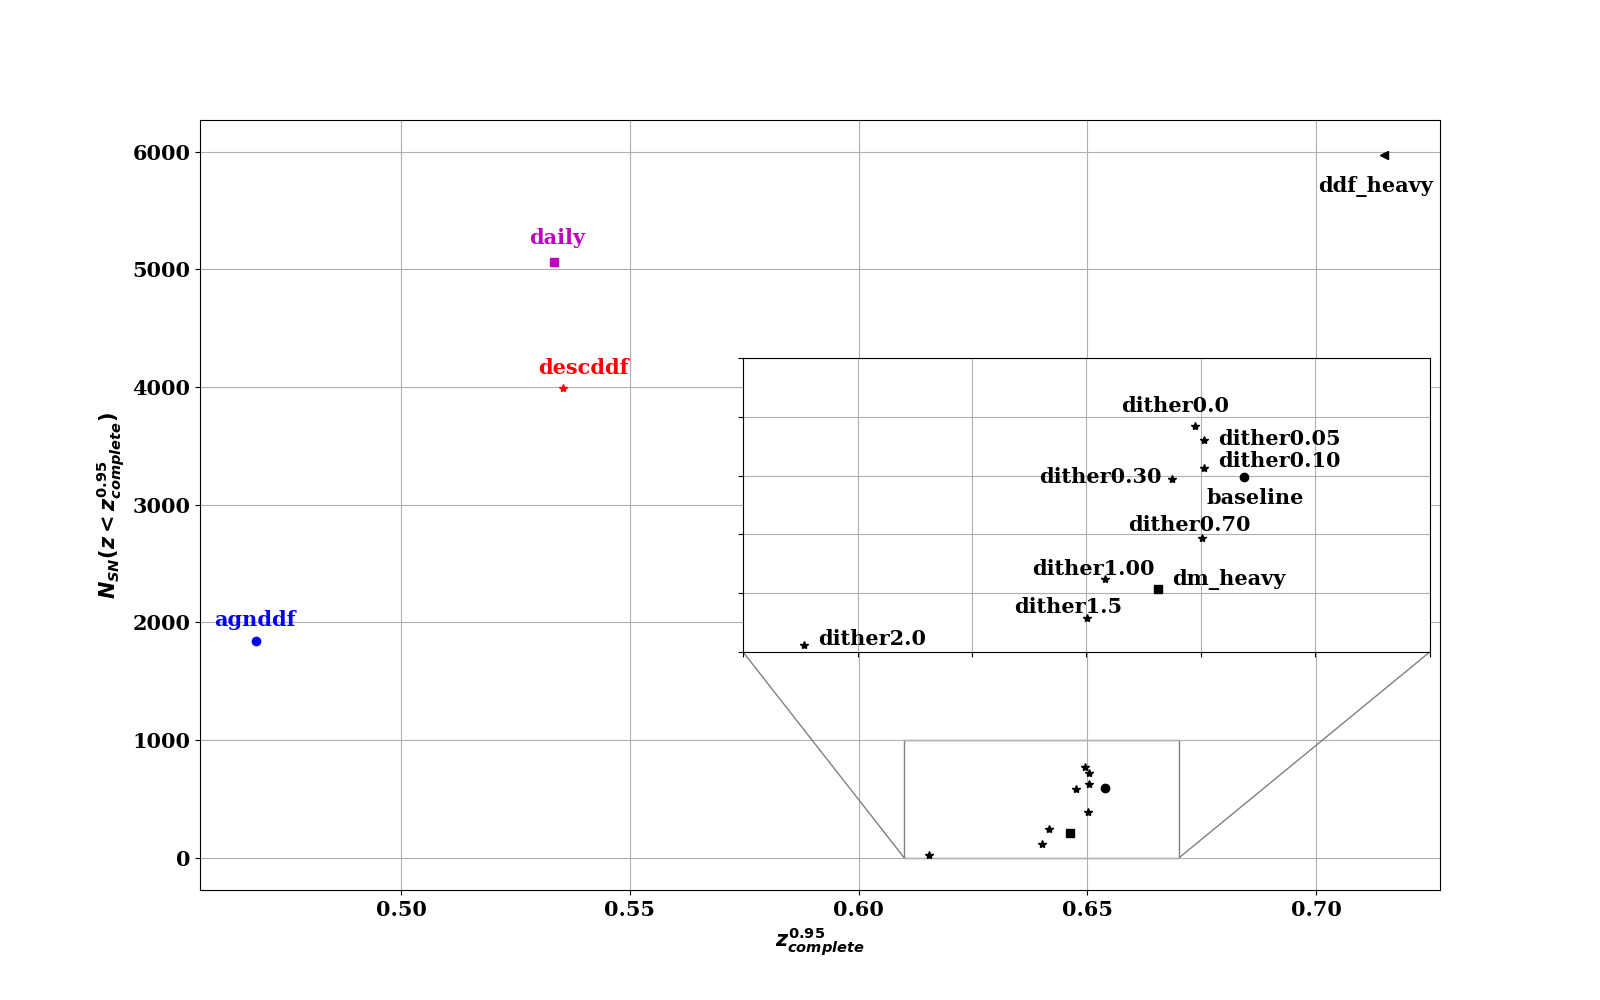
\includegraphics[width=1.\textwidth]{nsn_zlim_zoom.png}
 \caption{\nsncomp~vs \zcompb~for the observing strategies considered in this paper.}\label{fig:nsn_zlim_zoom}
\end{center}
\end{figure}

\par
The translationnal dithering is expected to affect both the number of well-sampled supernovae and the redshift of completeness for each of the pixel of a field. With no dithering, \nsncomp~and \zcompb~distributions are uniform on the whole field area. The dithering tends increase the cadence of observation and to decrease both \nsncomp~and \zcompb~(per pixel). The dithered pointings of the telescope are estimated from the central location of the fields (Tab. \ref{tab:locddf}) and lead to a distribution map of the metrics decreasing as the (pixel) distance to the central location increases. A more subtle effect is observed (Fig. \ref{fig:dither}) when all the pixel are considered to estimate (\sumnsncomp, \zcompb). It depends both on the cadence and on \nvisits. \zcompb~tends to decrease with an increase of the translationnal dither offset (\doffset), with a greater effect for low cadences. The total number of supernovae systematically decreases with \doffset~for high cadences. For low cadences, \sumnsncomp~tends to increase with \doffset~up to a maximum value (cadence dependent) and then decreases. This beheaviour is to be explained by two opposite effects in the estimation of \sumnsncomp: a decrease of the cadence and an increase of the survey area with \doffset.

\begin{figure}[htbp]
  \begin{center}
  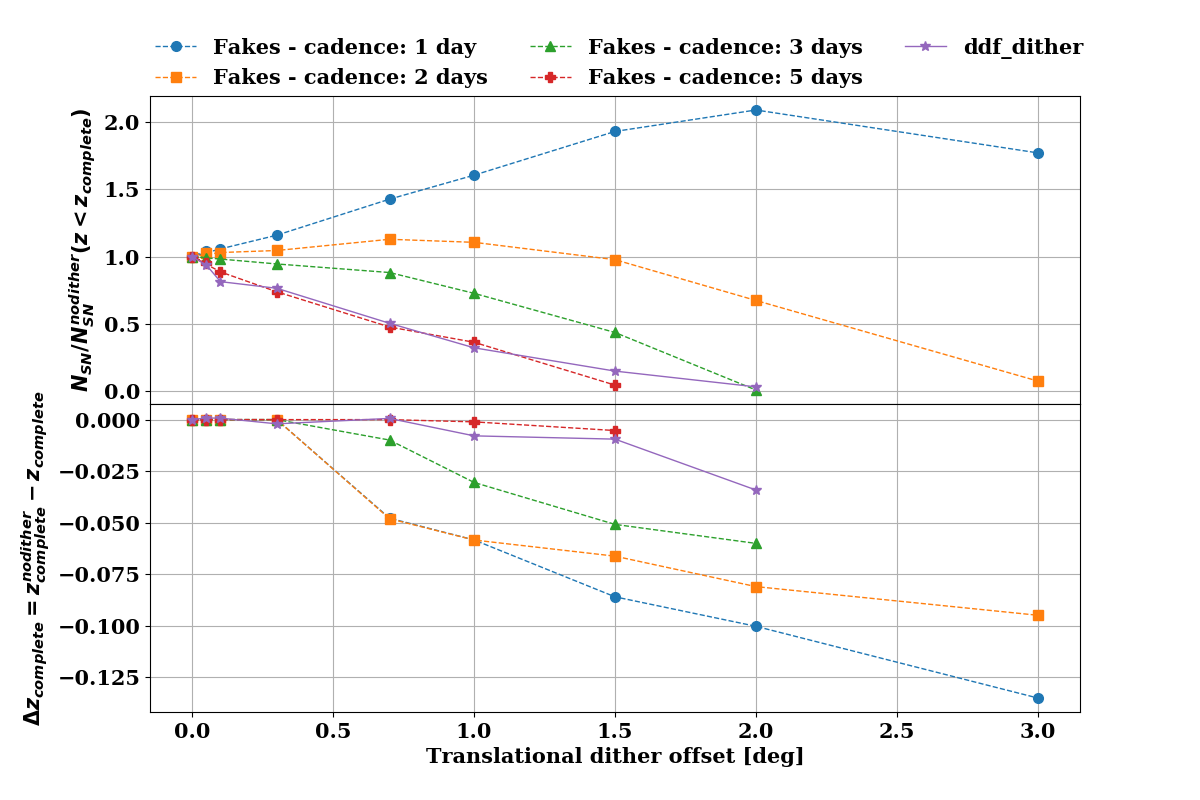
\includegraphics[width=0.9\textwidth]{dither_ddf.png}
 \caption{Ratio of the number of supernovae $N_{SN}/N_{SN}^{nodither}$ (top) and \zcompb~difference (bottom) as a function of translationnal dither offset. The simulations labelled as 'Fakes' (dotted lines) correspond to regular cadences (1,2,3,5 days) with median observing conditions (5$\sigma$ depth single exposure: 24.13/23.84/23.45/22.74/22.10 for $g/r/i/y/z$ bands, respectivelly.}\label{fig:dither}
\end{center}
\end{figure}



\section{Towards an optimization of the number of visits}
\label{sec:opti}

The analysis of the most recent simulations have shown (see Sec. \ref{sec:analysis}) that it was difficult, with the proposed cadences of observation, filter allocation and season lengths, to collect complete samples of \sne~with redshift higher than \zcompb\seq 0.55-0.6 for a DD budget of \seq 5\per.  %A high budget (\seq 13.5\per) is requested to reach \zcompb\seq 0.65.
The redshift limits are mainly driven by \sumnvisitsb$\times$ cadence. With optimal survey parameters (i.e. a regular cadence of observation of one day, no dithering, minimal fluctuation of observing conditions) the depth of the four families considered in Sec. \ref{sec:analysis} would be \zcompb $\sim$ (0.77,0.59,0.54,0.72) for (\osfamily{baseline},\osfamily{agn},\osfamily{daily},\osfamily{desc}), respectivelly. These values are well below the ambitious goal of \zcompb\seq1. According to Eq. \ref{eq:zlimsnr} the only way to reach higher redshift limits is to increase the minimal SNR requested in each band that is, in turn, the number of visits. We present in this section a method of defining the relationship between the redshift limit and the number of visits per band and per observing night (for a defined cadence). 
\par
As described in Eq. \ref{eq:ddbudget} the DD budget depends primarily on 5 parameters: the number of fields to observe, the season length (per field and per season), the number of seasons of observation, the cadence of observation (per field and per season), and the number of visits \nvisitsb~per filter and per observing night. \nvisitsb~affect \snrb~through the flux measurement uncertainties  $\sigma_i^b$. In the background-dominated regime one has $\sigma_i^b \simeq \sigma_5^b$ where $\sigma_5^b$ is equal by definition to
\begin{equation}
  \begin{aligned}
    \sigma_5^b &=  \frac{f_5^b}{5}
    \end{aligned}
\end{equation}
where $f_ 5^b$ is the five-sigma flux related to the five-sigma depth magnitude $m_5^b$ through:
\begin{equation}
  \begin{aligned}
    m_5^b &= -2.5 \log f_5^b+zp^b
    \end{aligned}
\end{equation}
where $zp^b$ is the zero point of the considered filter.  $m_5^b$ is related to \nvisitsb through:
\begin{equation}
  \begin{aligned}
    m_5^b - m_5^{b, single~visit} & =  1.25 \log(N_{visits}^b)
    \end{aligned}
  \label{eq:opt4}
\end{equation}
where $m_5^{b, single~visit}$ is the five-sigma depth corresponding to a single visit, a parameter depending on observing conditions. These equations \eqref{eq:opt1}-\eqref{eq:opt4} describe the relationship between \snrb~ and \nvisitsb. The request $\snrb~\geq~\snrbmin$ is equivalent to $\nvisitsb~\geq~\nvisitsbmin$ and equ. \eqref{eq:zlimsnr} may be written:
\begin{equation}
  \begin{aligned}
    \zlim &\Longleftarrow & \sigc \leq 0.04 & \Longleftarrow &\cap (\nvisitsb~\geq~\nvisitsbmin)
    \end{aligned}
 \label{eq:zlimnvisits}
\end{equation}
\\
The relations \eqref{eq:zlimsnr} and \eqref{eq:zlimnvisits} are not univocal. A lot of \snrb~combinations lead in fact to the same result and constraints have to be applied to choose the optimal configuration. We have performed a systematic scan of the SNR parameter space (\snrg,\snrr,\snri,\snrz,\snry) and picked combinations with \sigc$\simeq$0.04.  The optimal solution is selected by minimizing the total number of visits per observing night and by fixing a maximum number of visits in the y-band (namely \nvisitsy$\leq$20). This selection aims at reducing the systematic (potentially severe) effects of the \by~band. The result is displayed on Fig. \ref{fig:nvisits_zlim} for a 1 day cadence. 

\begin{figure}[htbp]
\begin{center}
  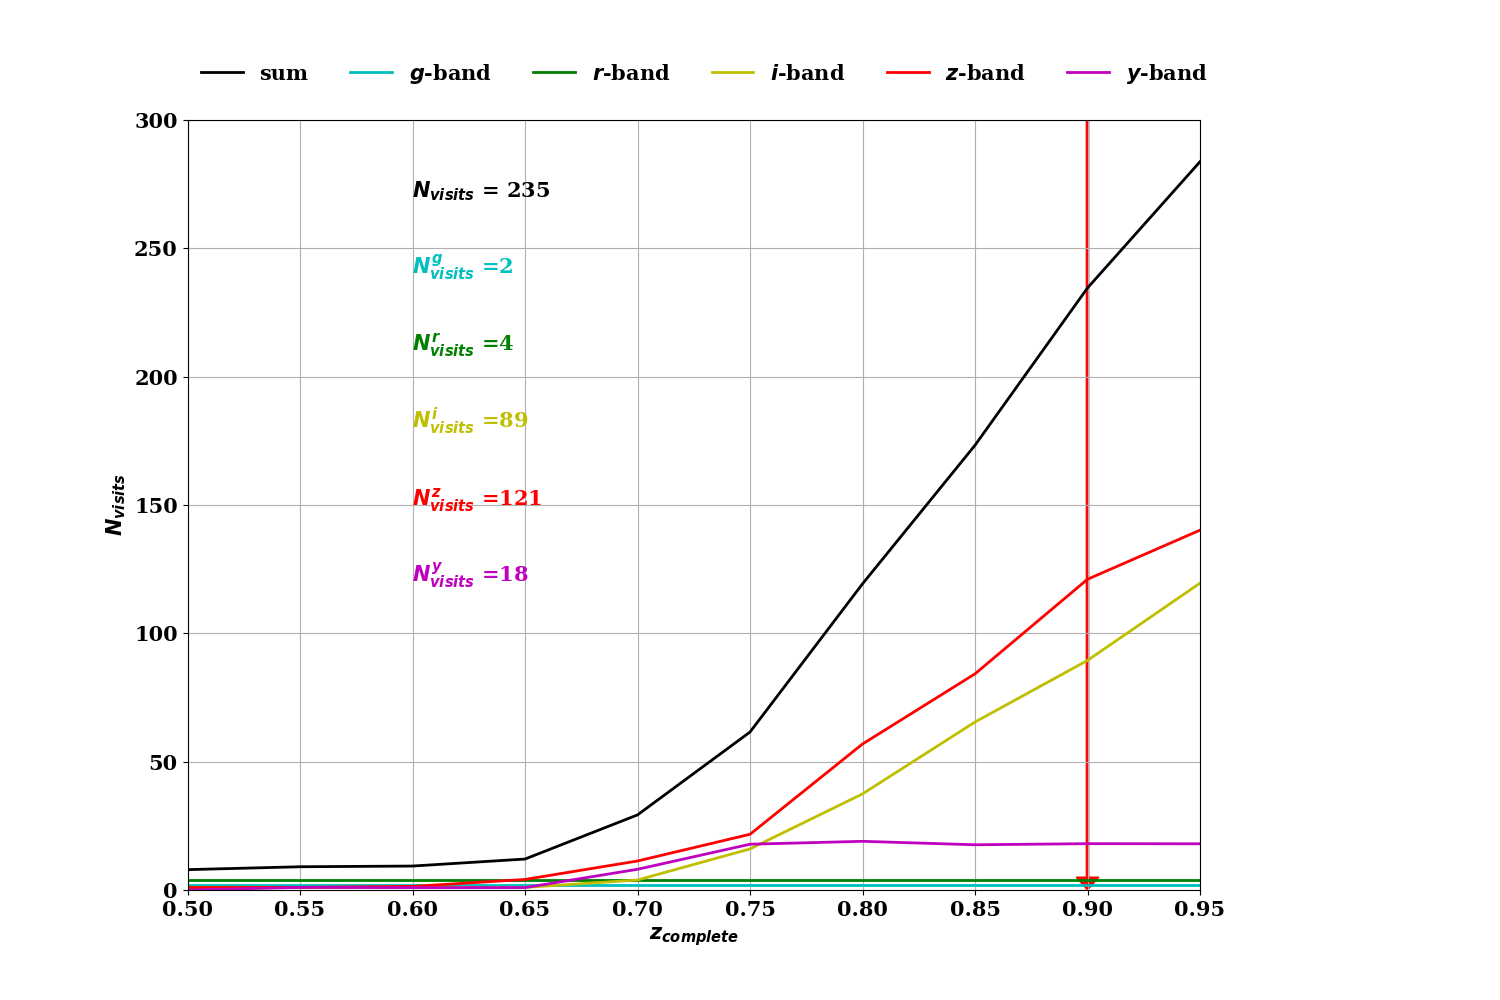
\includegraphics[width=0.95\textwidth]{nvisits_zlim.png}
 \caption{Number of visits as a function of the completeness redshift. 250 visits {\it with} the following filter allocation (\nvisitsall)=(2,2,98,130,18) are requested per observing night to reach \zcomp\seq0.9 for a cadence of one day.}\label{fig:nvisits_zlim}
\end{center}
\end{figure}

\begin{comment}
We may then use \ref{eq:zliminvisits} and \ref{fig:nvisits_zlim} to estimate the redshift of completeness corresponding to the number of visits of \ref{tab:ddbudget}. The conclusions of the result (Tab. \ref{tab:zlim}) are (a) it is very difficult to reach completeness redshifts higher than 0.6-0.7 if all fields are observed for ten years ; (b) the only way to explore higher  redshift domains is to reduce the number of seasons of observation.

\begin{table}[!htbp]
  \caption{Redshift of completeness as a function of the DD budget and the cadence of observation for a configuration of 5 fields. The first/second number corresponds to 10/2 seasons of observation per field. The redshift of completeness are independent on the cadence since the total SNR per band, \snrb,are identical.}\label{tab:zlim}
  \begin{center}
    \begin{tabular}{c|c|c|c}
      \hline
      \hline
      \diagbox[innerwidth=3.cm,innerleftsep=-1.cm,height=3\line]{budget}{cadence} & 1 & 2 & 3\\
      \hline
      6\% &\multicolumn{3}{c}{0.62/0.74} \\
      10\% & \multicolumn{3}{c}{0.66/0.79} \\
      15\% & \multicolumn{3}{c}{0.68/0.83}\\
      \hline
    \end{tabular}
  \end{center}
\end{table}
\end{comment}

\section{Rolling Deep Drilling surveys to reach \zcomp~domains}
\label{sec:scenario}
\paragraph{Season length and field location}
The season length of observation is a parameter involved in the estimation of the budget and the number of well-sampled \sne.  It depends on the position of the field (w.r.t. LSST position) but also on the number of visits per night. The season length may be estimated from a list of night during which a field is visible (i.e. with altitude 20$^o\leq$ alt$\leq$86.5$^o$ and airmass$\leq$1.5) for a duration corresponding to \nvisits.  The results is given on Fig. \ref{fig:seasonlength_nvisits}. The season lengths decrease from 275-200 to 150-100 days for \nvisits~increasing from 1 to 400.  Combining information of sec. \ref{sec:opti} and Fig. \ref{fig:seasonlength_nvisits} lead to the conclusion that low cadences are favored to reach higher \zcomp~values while maximizing the season length.
%This is due to the fact that the minimal \snrb~to reach \zcomp~is independent on the cadence. The corresponding requested number of visits increases with the cadence. This leads to a decrease of the season length.

\begin{figure}[htbp]
\begin{center}
  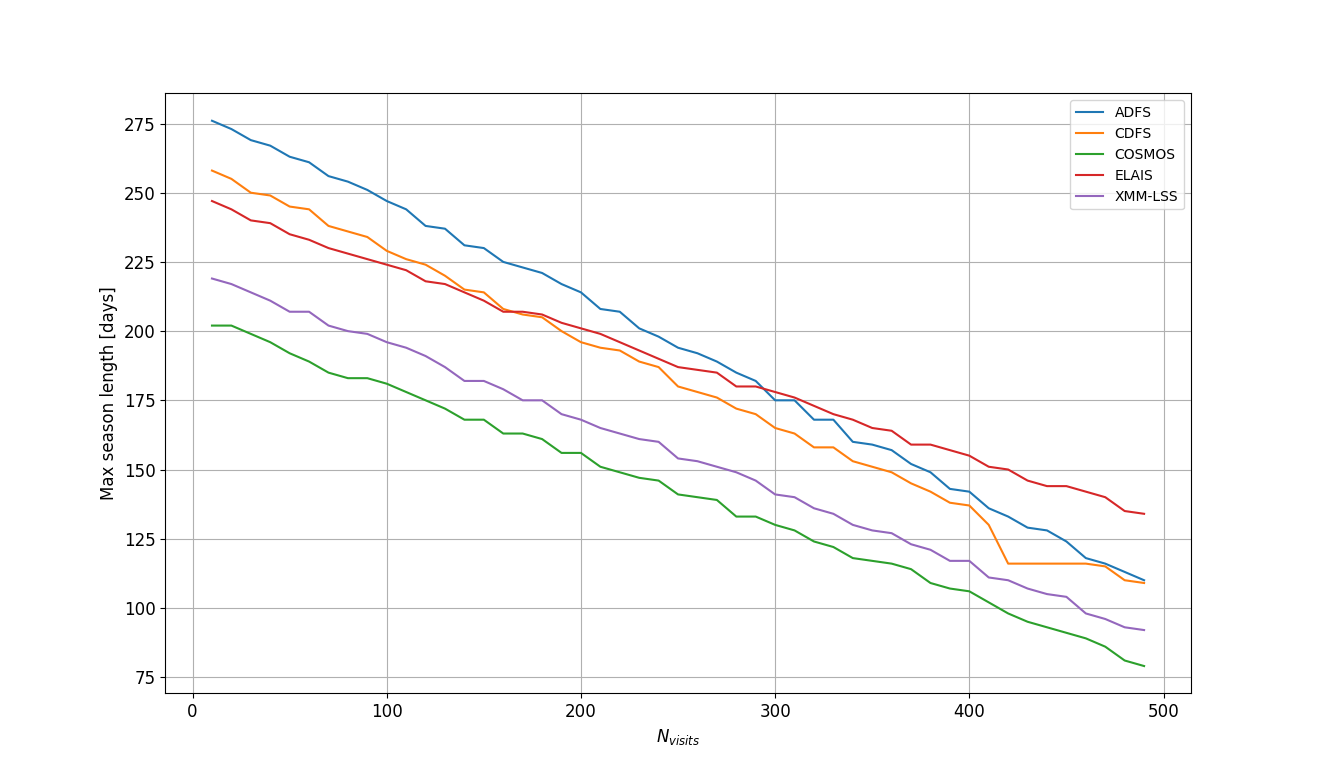
\includegraphics[width=0.95\textwidth]{seasonlength_nvisits.png}
 \caption{Maximal season length as a function of the number of visits.}\label{fig:seasonlength_nvisits}
\end{center}
\end{figure}

\subsection{Rolling Deep Drilling strategy}
A Deep Drilling program may be defined by the following parameters: number of fields to observe, number of season of observation (per field), season length (per field and per season),  number of visits per filter per observing night, DD budget, number of supernovae, and redshift of completeness.  Once the field parameters configuration (fields to observe, number of seasons, season length) is set, one of the three parameters (\zcomp, budget, \nvisits) may be fixed to estimate the two others using the results of Fig.~\ref{fig:nvisits_zlim}. 
\begin{comment}
A GUI (Fig. \ref{fig:budget_gui}) was designed from the results of sec. \ref{sec:opti} to design Deep Drilling scenarios. Once the field parametersconfiguration (fields to observe, number of seasons, season length) is set, one of the three parameters (\zcomp, budget, \nvisits) may be fixed to estimate the two others. 

\begin{figure}[htbp]
\begin{center}
  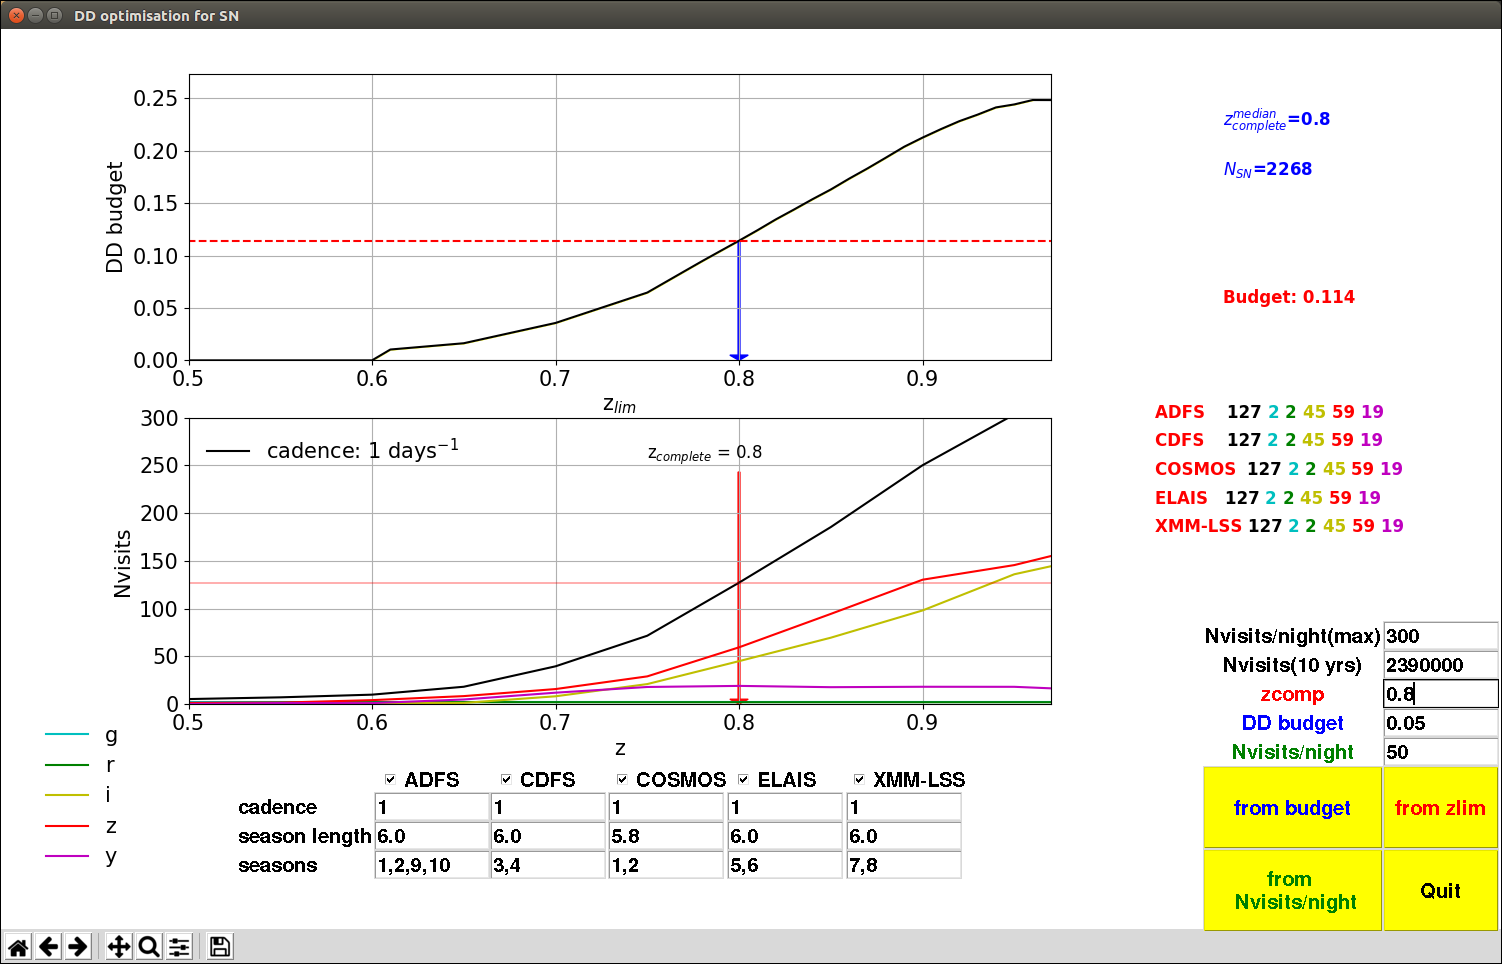
\includegraphics[width=0.95\textwidth]{budget_GUI.png}
 \caption{A GUI to define Deep Drilling programs. The field parameters (fields to observe, number of seasons, season length) are defined in the bottom table. The bottom plot displays the number of visits as a function of \zcomp. The budget as a function of \zcomp~is represented on the top plot. One of the three parameters (\zcomp, budget, \nvisits) may be fixed to estimate the two others. The expected total number of supernovae is also estimated. We have chosen \zcomp$\sim$0.8 as an illustraion.}\label{fig:budget_gui}
\end{center}
\end{figure}
\end{comment}

Observing 5 fields for ten years up to \zcomp $\sim$ 0.9 would certainly give access to a large sample of well-measured \sne~(around 11k) but also to an unrealistic scenario (DD budget: 87\%). The only way to reach higher \zcomp~while maintaining a reasonable budget is to reduce the number of seasons of observation. This is the purpose of the Deep Drilling Rolling (DDR) strategy characterized by a limited number of seasons of observation per field (typically 2) and a large number of visits per observing night (more than 200 for higher \zcomp).

\par
Building a consistent DDR strategy is not only a matter of adjusting LSST survey settings to stay within a reasonable budgetary envelope. Synergistic datasets from cosmological endeavors overlapping with LSST in area and timing are essential for the success of the supernovae program. Spectroscopy provides enormous added benefits through (a) the follow-up of the full sample of well-measured supernovae (photometric classification), and (b) the measurement of host-galaxy redshifts with high accuracy.
\par
Two of the spectroscopic resources contemporaneous with LSST, Primary Focus Spectrograph (PFS \cite{Tamura_2016}) and 4MOST(\cite{}), may provide guidance in the choice of the depth of the DDR survey. Two sets of fields may then be defined to fully benefit from the synergy with PFS and 4MOST: ultra-deep fields (\cosmos,\xmm), with \zcompb$\geq$0.9, and the follow-up/host-galaxy redshifts measurements would be performed by PFS; deep fields (\cdfs, \elais, \adfs), with spectroscopic measurements provided by TiDES. The redshift completeness for the deep fields will depend on the redshift range of the data provided by TiDES and on the DD budget of LSST. 




\begin{figure}[htbp]
\begin{center}
  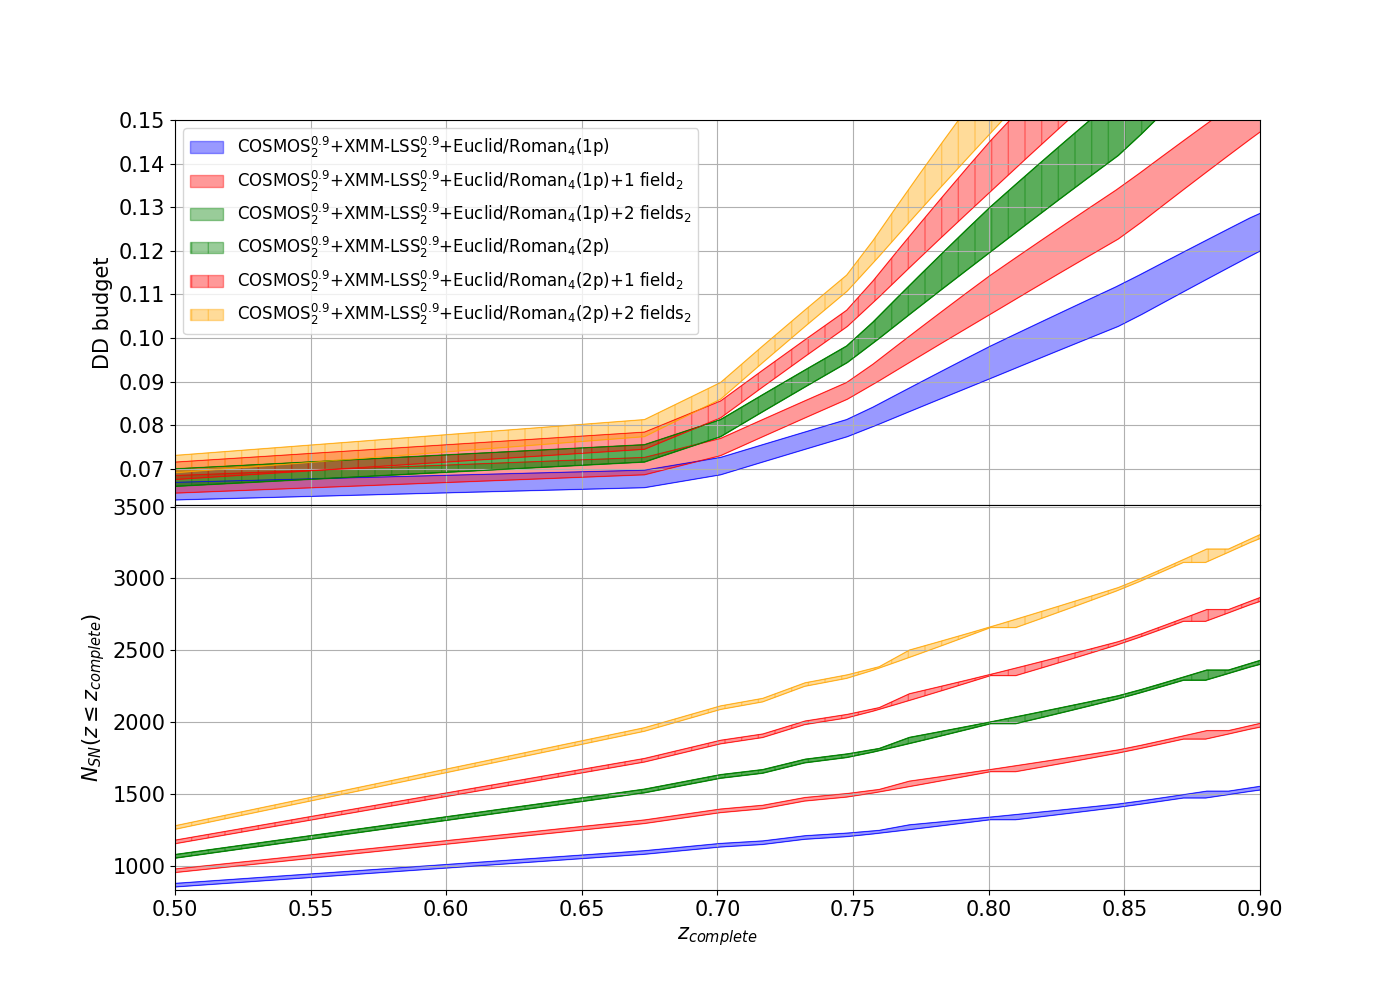
\includegraphics[width=0.9\textwidth]{budget_zcomp.png}
  \caption{DD budget as a function of the redshift of completeness of deep fields for a set of scenarios where the redshift of completeness of ultra-deep fields (\cosmos~and \xmm) is set to 0.9. Subscripts correspond to the number of seasons of observation and superscripts to the redshift limit. ER stands for Euclid/Roman field. Highest \zcomp~values are reached for a minimal strategy composed of two seasons of observations of \cosmos~and \xmm~with a depth of 0.9 plus 4 seasons of observation of the \adfs~ field (1 pointing). Coloured areas correspond to a variation of the number of $y$-band visits (20$\leq N_{visits}^y \leq$ 80).}\label{fig:budget_zcomp}
\end{center}
\end{figure}
\par



\begin{comment}
\begin{table}[!htbp]
  \caption{Set of scenarios to reach higher \zcomp.}\label{tab:rolling_scenarios}
  \begin{center}
    \begin{tabular}{c|c|c|c|c|c|c|c}
      \hline
      \hline
      Scenario & \zcomp & \nsncomp & budget & \nvisits & fields & seasons & season length\\
                       &                 &                     &               & \bg/\br/\bi/\bz/\by &        & & [month] \\
      \hline
      \multirow{5}{*}{\ddfscen{a}} & \multirow{5}{*}{0.8} & \multirow{5}{*}{2270} & \multirow{5}{*}{11.4\per} & & COSMOS & 1,2 & 5.8 \\
         &       &          &                  &          & CDFS         & 3,4 & 6.0 \\
         &       &          &                  &      127               & ELAIS        & 7,8 & 6.0 \\
         &       &          &                  &    2/2/45/58/19                  &XMM-LSS  & 9,10 & 6.0 \\
         &       &          &                  &                     &ADFS          & 1,2,5,6 & 6.0 \\
      \hline
      \multirow{5}{*}{\ddfscen{b}} & \multirow{5}{*}{0.84} & \multirow{5}{*}{2500} & \multirow{5}{*}{15.0\per} & & COSMOS & 1,2 & 5.4\\
         &       &          &                  &          & CDFS         & 3,4 & 6.0 \\
         &       &          &                  &      169               & ELAIS        & 7,8 & 6.0 \\
         &       &          &                  &    2/2/63/85/18                  &XMM-LSS  & 9,10 & 5.8\\
         &       &          &                  &                     &ADFS          & 1,2,5,6 & 6.0 \\
      \hline
      \multirow{3}{*}{\ddfscen{c}} & \multirow{3}{*}{0.9} & \multirow{3}{*}{1860} & \multirow{3}{*}{14.3\per} & & COSMOS & 1,2 & 4.7 \\
         &       &          &                  &     250     & CDFS         & 3,4 & 6.0 \\
         &       &          &                  &    2/2/98/130/18                 &ADFS          & 1,2,5,6 & 6.0 \\
      \hline
      \end{tabular}
  \end{center}
\end{table}
\end{comment}

% ----------------------------------------------------------------------

% ----------------------------------------------------------------------

%\section{Lessons from recent simulations}
%\label{sec:simu}

% ----------------------------------------------------------------------

\section{Discussion}
\label{sec:discussion}



% ----------------------------------------------------------------------

\section{Conclusion}
\label{sec:conclusion}



% ----------------------------------------------------------------------

\subsection*{Acknowledgments}

%%% Here is where you should add your specific acknowledgments, remembering that some standard thanks will be added via the \code{desc-tex/ack/*.tex} and \code{contributions.tex} files.

%This paper has undergone internal review in the LSST Dark Energy Science Collaboration. % REQUIRED if true

Author contributions are listed below. \\
Ph.~Gris: conceptualization,software,analysis,writing \\
N.~Regnault: conceptualization,writing \\
 % Standard papers only: author contribution statements. For examples, see http://blogs.nature.com/nautilus/2007/11/post_12.html

% This work used TBD kindly provided by Not-A-DESC Member and benefitted from comments by Another Non-DESC person.

% Standard papers only: A.B.C. acknowledges support from grant 1234 from ...

\input{desc-tex/ack/standard} % also available: key standard_short

% This work used some telescope which is operated/funded by some agency or consortium or foundation ...

% We acknowledge the use of An-External-Tool-like-NED-or-ADS.

%{\it Facilities:} \facility{LSST}

% Include both collaboration papers and external citations:
\bibliography{main,lsstdesc}

\end{document}

% ======================================================================
